\documentclass{article}
\usepackage{cmap}
\usepackage[utf8]{inputenc}
\usepackage[english,ukrainian]{babel}
\usepackage{graphicx}
\usepackage{geometry}
\usepackage{listings}
\usepackage{float}
\usepackage{multicol}
\usepackage{amsmath}
\geometry{
	a4paper,
	left=20mm,
	right=20mm,
	top=15mm,
	bottom=15mm,
}
\lstset{
	language=c,
	tabsize=4,
	keepspaces,
	showstringspaces=false,
}
\graphicspath{ {./pictures} }
\setlength{\parindent}{4em}

\newcommand\subject{Основи електроніки}
\newcommand\lecturer{професор кафедри ПЗ \\ Фечан А.В.}
\newcommand\teacher{доцент кафедри ПЗ \\ Коцун В.І.}
\newcommand\mygroup{ПЗ-22}
\newcommand\lab{7}
\newcommand\theme{Дослідження роботи аналого-цифрового і цифроаналогового перетворювачів}
\newcommand\purpose{Методом комп'ютерного моделювання дослідити роботу
	аналого-цифрового і цифро-аналогового перетворювачів та визначити похибку
	перетворення}

\begin{document}
\begin{normalsize}
	\begin{titlepage}
		\thispagestyle{empty}
		\begin{center}
			\textbf{МІНІСТЕРСТВО ОСВІТИ І НАУКИ УКРАЇНИ\\
				НАЦІОНАЛЬНИЙ УНІВЕРСИТЕТ "ЛЬВІВСЬКА ПОЛІТЕХНІКА"}
		\end{center}
		\begin{flushright}
			\textbf{ІКНІ}\\
			Кафедра \textbf{ПЗ}
		\end{flushright}
		\vspace{200pt}
		\begin{center}
			\textbf{ЗВІТ}\\
			\vspace{10pt}
			до лабораторної роботи № \lab\\
			\textbf{на тему}: “\textit{\theme}”\\
			\textbf{з дисципліни}: “\subject”
		\end{center}
		\vspace{112pt}
		\begin{flushright}
			
			\textbf{Лектор}:\\
			\lecturer\\
			\vspace{28pt}
			\textbf{Виконав}:\\
			
			студент групи \mygroup\\
			Коваленко Д.М.\\
			\vspace{28pt}
			\textbf{Прийняв}:\\
			
			\teacher\\
			
			\vspace{28pt}
			«\rule{1cm}{0.15mm}» \rule{1.5cm}{0.15mm} 2023 р.\\
			$\sum$ = \rule{1cm}{0.15mm}……………\\
			
		\end{flushright}
		\vspace{\fill}
		\begin{center}
			\textbf{Львів — 2023}
		\end{center}
	\end{titlepage}
		
	\begin{description}
		\item[Тема.] \theme.
		\item[Мета.] \purpose.
	\end{description}

	\section*{Індивідуальне завдання}
	\begin{enumerate}
		\item Запустити програму NI Multisim.  Зібрати схему представлену на рис. 2.
		\item Встановити параметри генератора на синусоїдальні коливання (рис. 3.) з частотою 1 Гц та амплітудою згідно зі своїм варіантом (табл. 1).
		
		\item Відкрити вікно Grapher View, та провести аналіз роботи АЦП-ЦАП перетворення. 
		\item Провести якісний аналіз відхилення перетвореного сигналу відносно вхідного. Результати представити у вигляді залежності, як показано на прикладі.
		\item Провести кількісний аналіз похибки перетворення. Для цього на генераторі встановити наступні параметри: синусоїдальні коливання з частотою 1 Гц та амплітудою згідно зі своїм варіантом. Для значень вхідної напруги Uвх (значення напруги на каналі осцилографа А) визначити значення вихідної (перетвореної) напруги Uвих (значення напруги на каналі осцилографа В). Отримані дані внести в таблицю. Розрахувати похибку вимірювання напруги згідно рівнянь (2) і (3).
		\item Дії описані в пункті 5 повторити для інших значень частот в межах від 1 Гц до 100 Гц . 
		\item Побудувати залежність точності перетворення від частоти.
		
	\end{enumerate}

	\section*{Хід виконання}
	
	\begin{figure}[H]
		\centering
		\includegraphics[width=\textwidth]{1}
		\caption{Схема 1}
	\end{figure}

	\begin{figure}[H]
		\centering
		\includegraphics[width=\textwidth]{2}
		\caption{Осцилограма 1 для схеми 1}
	\end{figure}

	\begin{figure}[H]
		\centering
		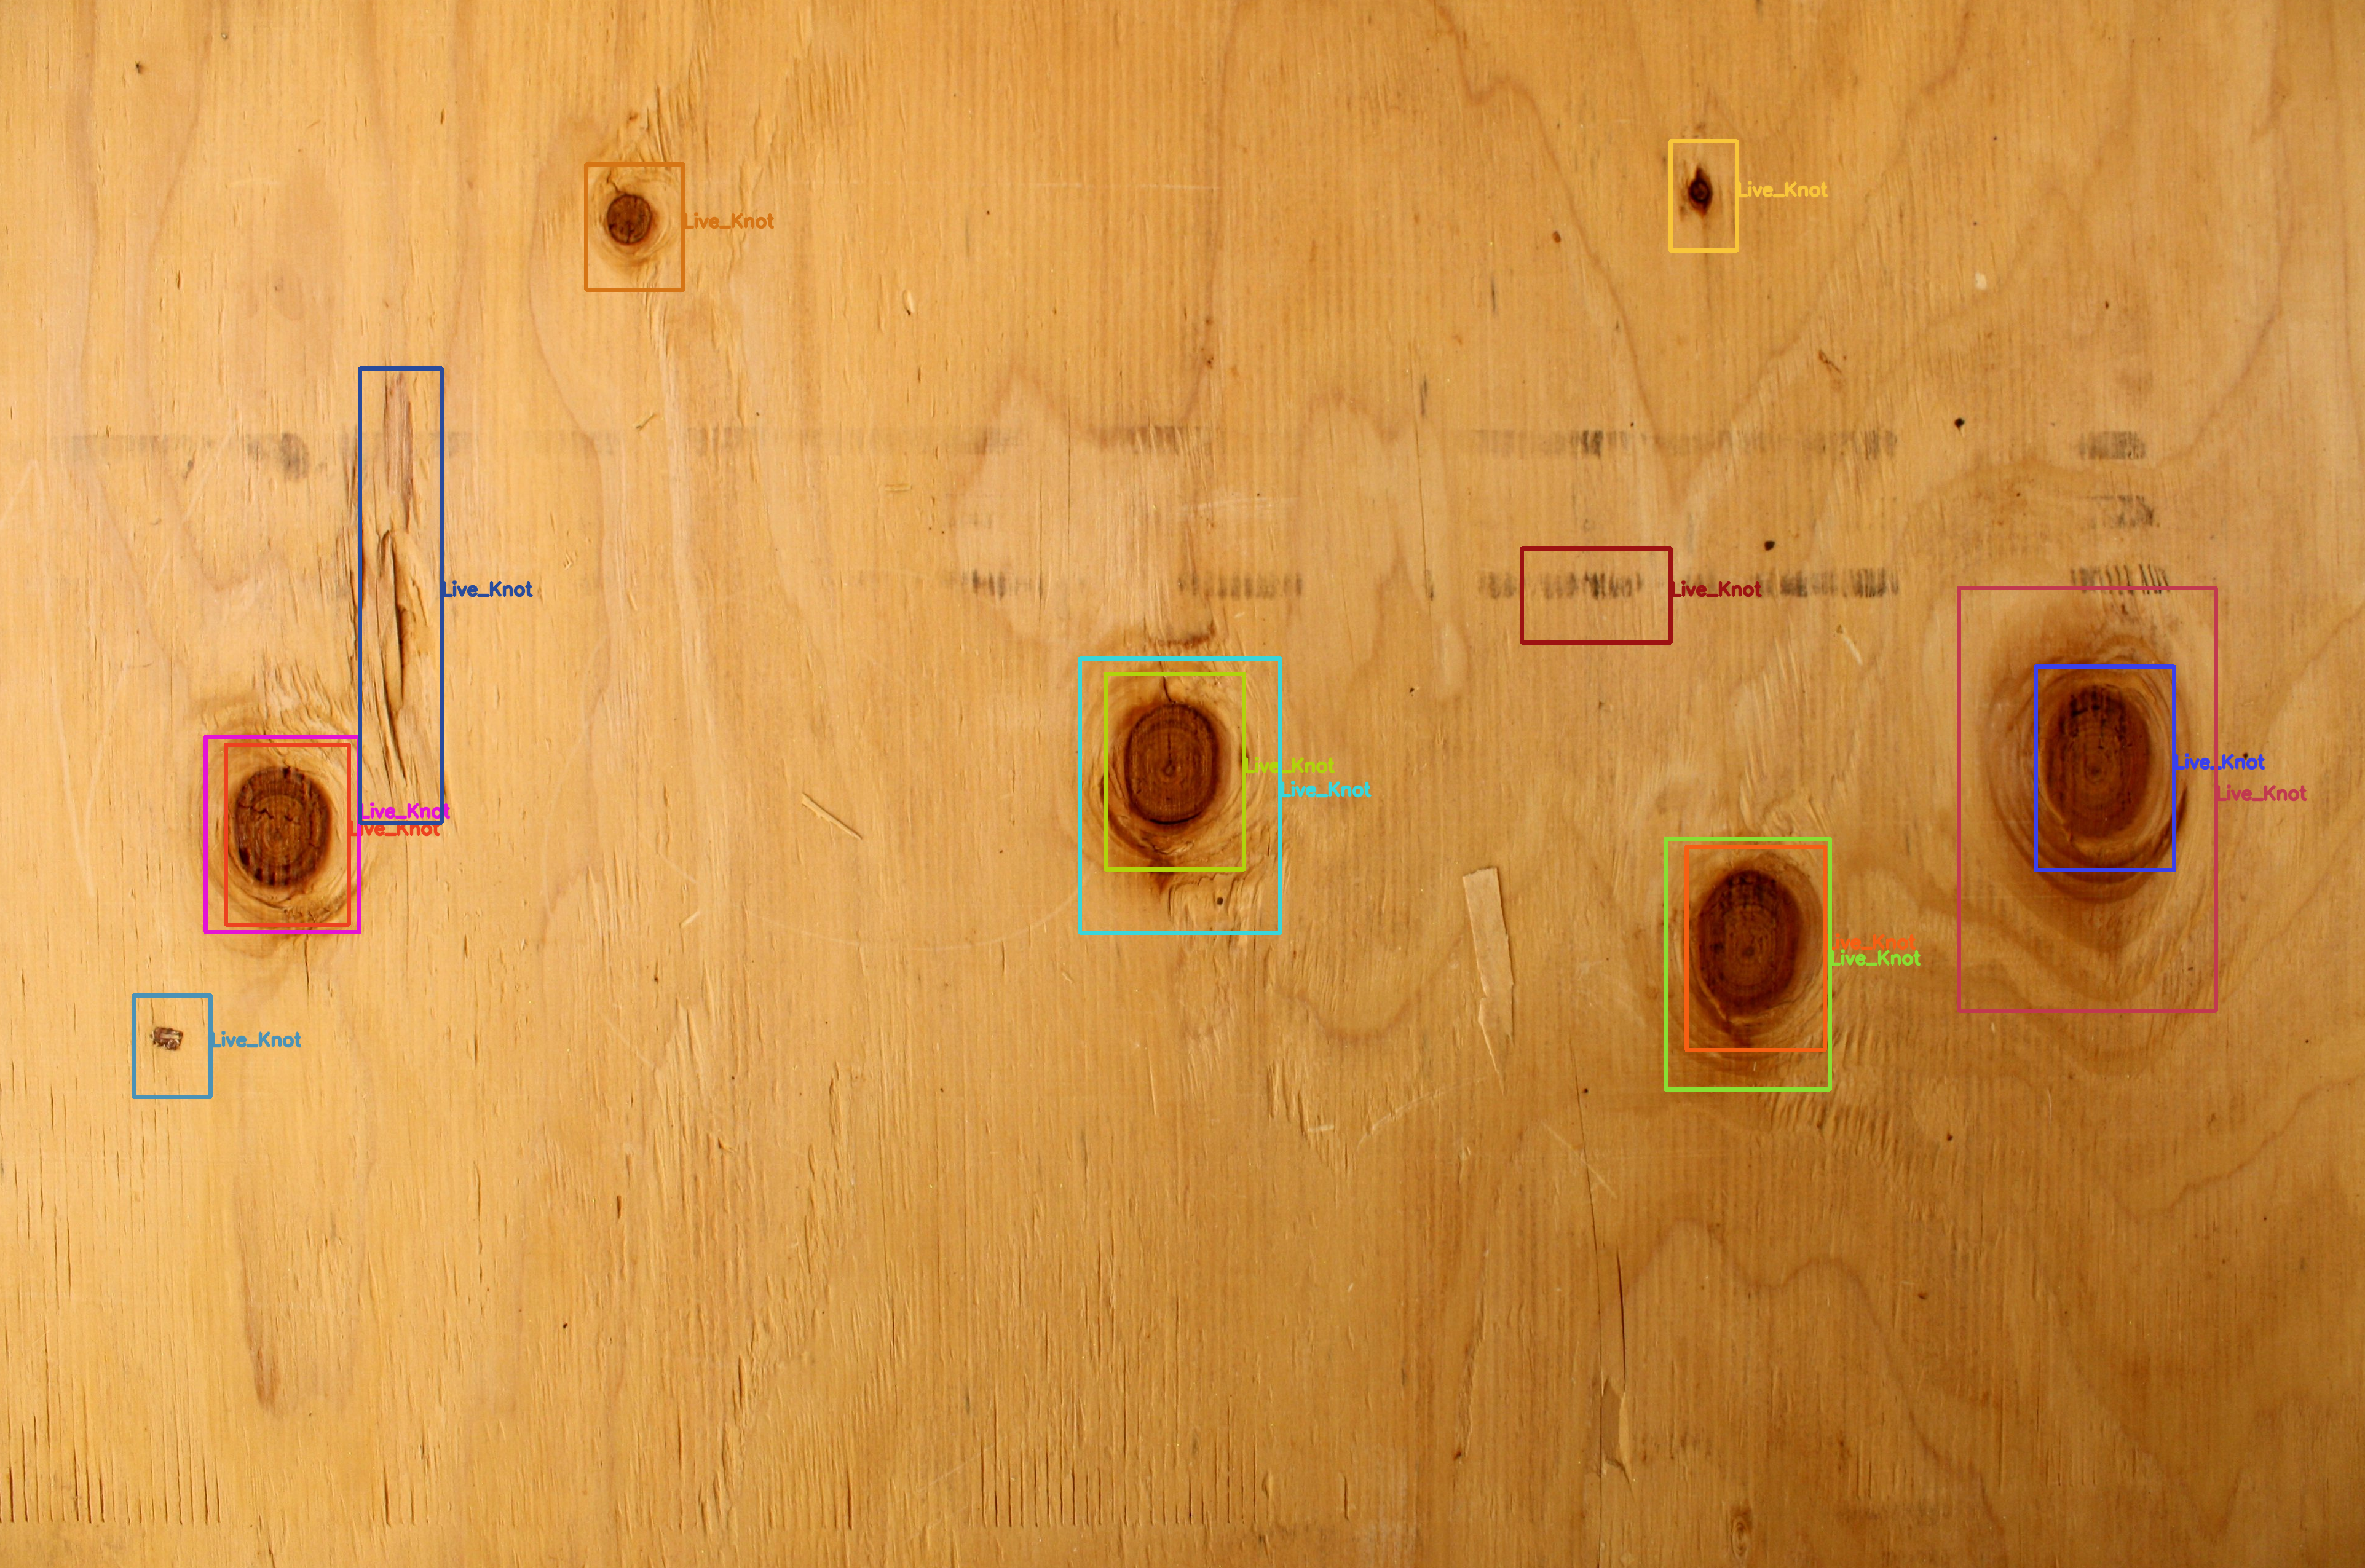
\includegraphics[width=\textwidth]{3}
		\caption{Осцилограма 2 для схеми 1}
	\end{figure}

	\begin{table}[H]
		\centering
		\renewcommand*\arraystretch{1.3}
		\begin{tabular}{|c|c|c|c|c|c|c|c|}
			\hline
			\multicolumn{4}{|c|}{\textbf{$1$ $Hz$}} & \multicolumn{4}{c|}{\textbf{$10$ $Hz$}} \\
			\hline
			\textbf{$U_{\text{вх}}$} & \textbf{$U_{\text{вих}}$} & \textbf{$\Delta U$} & \textbf{$\Delta U$ (\%)} & \textbf{$U_{\text{вх}}$} & \textbf{$U_{\text{вих}}$} & \textbf{$\Delta U$} & \textbf{$\Delta U$ (\%)} \\
			\hline
			1.36&1.28&0.058&5.88&1.85&1.64&0.11&11.35\\
			\hline
			2.36&2.22&0.05&5.93&4.44&4.1&0.07&7.65\\
			\hline
			4.93&4.80&0.02&2.63&6.07&5.85&0.03&3.62\\
			\hline
		\end{tabular}
	\end{table}

	\begin{table}[H]
		\centering
		\renewcommand*\arraystretch{1.3}
		\begin{tabular}{|c|c|c|c|c|c|c|c|}
			\hline
			\multicolumn{4}{|c|}{\textbf{$30$ $Hz$}} & \multicolumn{4}{c|}{\textbf{$50$ $Hz$}} \\
			\hline
			\textbf{$U_{\text{вх}}$} & \textbf{$U_{\text{вих}}$} & \textbf{$\Delta U$} & \textbf{$\Delta U$ (\%)} & \textbf{$U_{\text{вх}}$} & \textbf{$U_{\text{вих}}$} & \textbf{$\Delta U$} & \textbf{$\Delta U$ (\%)} \\
			\hline
			1.44&1.28&0.11&11.11&2.97&2.1&0.29&29.29\\
			\hline
			3.91&3.75&0.04&4.09&5.68&5.62&0.01&1.05\\
			\hline
			6.38&6.32&0.0&0.94&6.88&6.56&0.04&4.65\\
			\hline
		\end{tabular}
	\end{table}
	
	\begin{table}[H]
		\centering
		\renewcommand*\arraystretch{1.3}
		\begin{tabular}{|c|c|c|c|c|c|c|c|}
			\hline
			\multicolumn{4}{|c|}{\textbf{$70$ $Hz$}} & \multicolumn{4}{c|}{\textbf{$100$ $Hz$}} \\
			\hline
			\textbf{$U_{\text{вх}}$} & \textbf{$U_{\text{вих}}$} & \textbf{$\Delta U$} & \textbf{$\Delta U$ (\%)} & \textbf{$U_{\text{вх}}$} & \textbf{$U_{\text{вих}}$} & \textbf{$\Delta U$} & \textbf{$\Delta U$ (\%)} \\
			\hline
			4.04&2.92&0.27&27.72&6.44&4.1&0.36&36.36\\
			\hline
			6.12&5.39&0.11&11.92&6.98&6.56&0.06&6.01\\
			\hline
			6.95&6.67&0.04&4.02&1.3&4.1&2.15&215\\
			\hline
		\end{tabular}
	\end{table}
	
	\begin{figure}[H]
		\centering
		\includegraphics[width=\textwidth]{4}
		\caption{Графік залежності  точності перетворення від частоти}
	\end{figure}
	
	\section*{Висновки}
	Під час виконання лабораторної роботи я методом комп'ютерного моделювання дослідив роботу
	аналого-цифрового і цифро-аналогового перетворювачів та визначив похибку
	перетворення.
	    
\end{normalsize}
\end{document}
